% !TeX program = pdfLaTeX
\documentclass[12pt]{article}
\usepackage{amsmath}
\usepackage{amsthm}
\usepackage{graphicx,psfrag,epsf}
\usepackage{enumerate}
\usepackage{natbib}
\usepackage{booktabs}
\usepackage{longtable}
\usepackage{array}
\usepackage{adjustbox}
\usepackage{multirow}
\usepackage{subfig}
\usepackage[table]{xcolor}
\usepackage{wrapfig}
\usepackage{float}
\usepackage{colortbl}
\usepackage{hyperref}
\usepackage{pdflscape}
\usepackage{tabu}
\usepackage{threeparttable}

\usepackage{verbatim}
\usepackage{url} % not crucial - just used below for the URL

%\pdfminorversion=4
% NOTE: To produce blinded version, replace "0" with "1" below.
\newcommand{\blind}{0}

% DON'T change margins - should be 1 inch all around.
\addtolength{\oddsidemargin}{-.5in}%
\addtolength{\evensidemargin}{-.5in}%
\addtolength{\textwidth}{1in}%
\addtolength{\textheight}{1.3in}%
\addtolength{\topmargin}{-.8in}%

\newenvironment{definition}[1]% environment name 
{% begin code 
  \par\vspace{.75\baselineskip}\noindent 
  \textbf{Definition (#1)}\begin{itshape}% 
  \par\vspace{.5\baselineskip}\noindent\ignorespaces 
}% 
{% end code 
  \end{itshape}\ignorespacesafterend 
}

\providecommand{\tightlist}{%
  \setlength{\itemsep}{0pt}\setlength{\parskip}{0pt}}

\begin{document}

\def\spacingset#1{\renewcommand{\baselinestretch}%
{#1}\small\normalsize} \spacingset{1}


%%%%%%%%%%%%%%%%%%%%%%%%%%%%%%%%%%%%%%%%%%%%%%%%%%%%%%%%%%%%%%%%%%%%%%%%%%%%%%


\if0\blind
{
  \title{\LARGE\bf Adapting the Chumbley Score to match striae on Land Engraved Areas (LEAs) of bullets}
  \maketitle
} \fi

% \if1\blind
% {
%   \bigskip
%   \bigskip
%   \bigskip
%   \begin{center}
%     {\LARGE\bf Adapting the Chumbley Score to match striae on Land Engraved Areas}
%   \end{center}
%   \medskip
% } \fi

\bigskip
\begin{abstract}
The same-source problem remains a major challenge in forensic toolmark
and firearm examination. Technological advances in surface imaging allow
measurements of 3D surfaces at previously unforeseen resolutions and
enable digitized imaging. Here, we investigate the applicability of the
Chumbley scoring method \citep{hadler}, developed for screwdriver
markings, for same-source identification of bullet striae. We provide
methods to identify parameters that minimize the error rates for
matching of LEAs using Hamby datasets 44 and 252 measured by NIST and
CSAFE. We suggest a remedial algorithm to alleviate the problem of
failed tests in the method, increasing both the power of the test and
reducing error rates. Type II error rates of the proposed method improve
by more than one third (Type I error of 0.05) and are on average about
0.22. This puts the proposed method on similar footing as other single
feature matching approaches in the literature.
\end{abstract}

\noindent%
{\it Keywords:} forensic science, toolmark, cross-correlation, Mann-Whitney U statistic, land engraved areas (LEAs), algorithm, signatures, same-source problem
\vfill

\newpage
\spacingset{1.45} % DON'T change the spacing!

\newcommand{\cited}[1]{{\textcolor{red}{#1}}}

\setlength\parindent{0pt}

\tableofcontents
\newpage

\section{Introduction}\label{introduction}

Same-source analyses are a major part of a Forensic Toolmark Examiner's
job. In current practice, examiners make these comparisons by visual
inspection under a comparison microscope and come to one of the
following four conclusions: identification, inconclusive, elimination or
unsuitable for examination \citep{afte-toolmarks1998}. These conclusions
are made on the basis of ``unique surface contours'' of the two
toolmarks being in ``sufficient agreement'' \citep{afte-toolmarks1998}.
AFTE describes the term ``sufficient agreement'' as the possibility of
another tool producing the markings under comparison, as practically
impossible \citep{afte-toolmarks1998}. Potential subject bias in the
assessment as well as the lack of specified error rates are the main
points of criticisms first raised by the National Research Council in
2009 \citep{NAS:2009} and later emphasized further by the President's
Council of Advisors on Science and Technology \citep{pcast2016}.

Technological advances, such as profilometers and confocal microscopy
allow to measure 3D surfaces in a high-resolution digitized form. This
technology has become more accessible over the last decade, and has made
its way into topological images of ballistics evidence, such as bullet
lands and breech faces
\citep{DeKinder1, DeKinder2, Bachrach1, vorburger2016}. Digitized images
of 3D surfaces of form the data basis of statistical analysis of
toolmarks. A statistical approach based on data removes both
subjectivity from the assessment and allows a quantification of error
rates for both false positive and false negative identifications.

Methods for matching marks for a variety of tools have been studied in
the literature (see \autoref{tab:toolmarks-ER} for an overview):
\citet{manytoolmarks1} and \citet{chumbley} have been analyzing
screwdriver marks digitized using a profilometer; \citet{manytoolmarks2}
have investigated 3D marks from screwdriver, tongue and groove pliers
captured using a confocal microscope; \citet{afte-chumbley} have been
investigated digitized marks from slip-joint pliers generated by a
surface profilometer.

Analysis of these digitized markings require the use of statistical
methods which can quantify the scientific mechanism of comparing
markings and serve as basis for an error rate calculation.
\citet{manytoolmarks2} define a relative distance metric and use it as
similarity measure between two toolmarks. \citet{manytoolmarks1} extract
many small segments in the markings of two toolmarks and compare
similarity using a maximum Pearson correlation coefficient. The Chumbley
scoring method, first introduced by \citet{chumbley}, uses a similar but
more extensive framework based on a Mann-Whitney U test of the resulting
correlation coefficients. This approach is non-deterministic, because
segments are chosen randomly. \citep{hadler} make the score
deterministic for each pair of toolmarks by choosing segments for
comparison systematically. This approach also ensures independence
between segments of striae.

\begin{table}[ht]
\centering
\resizebox{\textwidth}{!}{\begin{tabular}{rlrrr}
  \hline
Research paper & Method & Data Source & False Positives & False Negatives\\
  \hline
 \textbf{\citet{manytoolmarks1}} & Maximum Pearson & Screwdrivers & & \\ & Correlation &  & - & - \\ \hline
 \textbf{\citet{chumbley}} & Randomized & Screwdrivers & & \\ (Same-Surface Same-Angle) & Chumbley Score & & 2.3\% & 8.9\%  \\ \hline
  \textbf{\citet{afte-chumbley}} & Randomized & Slip-joint  &  & \\ & Chumbley Score &  & - & - \\ \hline 
  \textbf{\citet{hadler}} & Deterministic & Screwdrivers & & \\ (Same-Surface Same-Angle) & Chumbley Score & & 0\% & 6\%  \\ \hline
  \textbf{\citet{manytoolmarks2}} & Similarity Measure & Screwdrivers & & \\ (Different Surfaces-same angle) & Relative Distance Metric & & 5.9\% &  9.4\% \\ (Same Surfaces-same angle)&  & & 0.22\% &  0\% \\
   \hline
\end{tabular}}
\caption{\label{tab:toolmarks-ER} Error Rates in same-source toolmark analysis reported in the literature. The top four reported papers use some variation of the Chumbley-score method.}
\end{table}

In this paper, we are investigating the applicability of the Chumbley
scoring method by \citet{hadler} to assess striation marks on bullet
lands for same-source identification. Striation marks on bullets are
made by impurities in the barrel. As the bullet travels through the
barrel, these imperfections leave ``scratches'' on the bullet surface
(see top of \autoref{fig:rgl}). Typically, only striation marks in the
land engraved areas (LEAs) are considered \citep{afte-article1992}.
Bullet lands are depressed areas between the grooves made by the rifling
action of the barrel. Compared to toolmarks made by screwdrivers
striation marks on bullets are typically much smaller, both in length
and in width. Bullets also have a curved cross-sectional topography.

In same-source comparisons this curvature is usually removed using some
form of Gaussian filter \citep{ma2004} or non-parametric smoothing
\citep{aoas}. An overview of some of the error rates reported in the
literature on bullet matching is given in \autoref{tab:bullets-ER}.
\citet{chu2013} use an automatic method for counting consecutive
matching striae (CMS). The authors report an error rate of 52\% for
known same-source land comparisons to be (incorrectly) identified as
different-source (false negative) and zero false positives for known
different-source lands. \citet{ma2004} and \citet{vorburger2011} discuss
CCF (cross-correlation function) and its discriminating power and
applicability for same-source analyses of bullets, but do not provide
any error rates in their discussion. \citet{aoas} use multiple features,
such as CCF, CMS, D (distance measure), etc. in a random forest based
method and compare every land against every other land of digitized
versions of Hamby 252 and Hamby 44 \citep{hamby} published on the NIST
Ballistics Database \citep{nist}. The authors report an out-of-bag
overall error rate of 0.46\%, comprised of an error rate of 30.05\% of
same-source pairs that were not identified and an error rate of 0.026\%
of different-source pairs that were incorrectly identified as
same-source.

\begin{table}[ht]
\centering
\resizebox{\textwidth}{!}{\begin{tabular}{rlrrr}
  \hline
Method & Data Source & False Positives & False Negatives\\
  \hline
  \textbf{\citet{aoas}} & LEAs \\
Consecutive Matching Bullets Striae (CMS) &  &  6.25\% &  33.85\% \\ 
Consecutive Non-matching Striae (CNMS)  & &  6.26\% & 35.42\%  \\ 
Average Distance (D) &   &   6.25\% & 45.83\% \\ 
Cross-correlation Function (CCF) & &  6.25\% & 17.71\%  \\ 
Sum of Peaks (S) &  &  6.25\% &  18.23\% \\
   \hline
   \textbf{\citet{chu2013}} & LEAs \\
Consecutive Matching Bullets Striae (CMS) &  &  0\% &  52\% \\ 
   \hline
   \textbf{\citet{chu2010}} \& \textbf{\citet{ma2004}} & LEAs \\
Cross-Correlation Function (CCF) &  &  - &  - \\ 
    \hline
\end{tabular}}
\caption{\label{tab:bullets-ER} Error Rates in same-source single feature land-to-land analysis reported in the literature.}
\end{table}

The Chumbley score provides us with another approach in the same-source
assessment of bullet striation marks. \citet{chumbley} compare two
toolmarks for same-source. The data for this study was obtained from 50
sequentially manufactured screwdriver tips. \citet{chumbley} report
error rates for markings made by the tips at different angles. For
markings made at 30 degree the authors report an average false negative
error rate of 0.089 and an average false positive error rate of 0.023.
For marks made under angles of 60 and 85 degrees, respectively, the
false negatives error rate is 0.09 while the rate of false positives
decreases to 0.01. The paper by \citet{hadler} is based on the same data
but the authors focus on markings made under the same angle. The error
rates associated with the deterministic version of the score are
reported as 0.06 for false negatives and 0 for false positives.

\begin{figure}
\centering
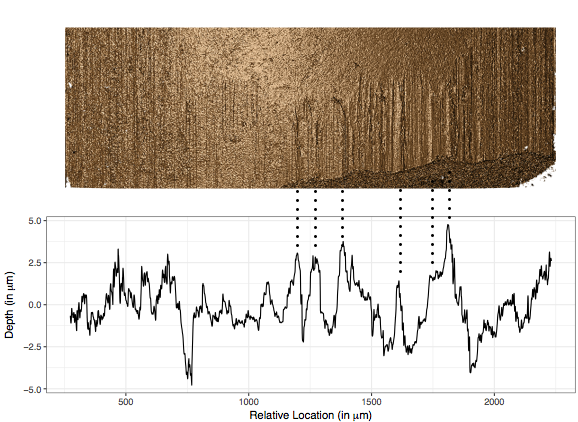
\includegraphics[width=\textwidth]{images/B6-B2-L6-rescaled.png}


\caption{\label{fig:rgl} Image of a bullet land from a confocal light microscope at 20 fold magnification (top) and a chart of the corresponding signature of the same land (bottom). The dotted lines connect some peaks visible in both visualizations.}

\end{figure}

In this paper we evaluate the adaptability of the Chumbley score as a
measure to quantify similarity in land engraved areas (LEAs) on bullets.
For that we briefly introduce the deterministic method suggested by
\citet{hadler} in section 2. In the process we provide methods to
identify parameters that minimize the error rates. We then investigate
persistent scenarios in which the method proposed by \citet{hadler}
fails to come to a result. We go on to provide a solution to the failed
tests problem, consequently increasing the power of the test and
reducing error rates in the process. We set up a testing framework to
compare the performance of the two algorithms in section 3 and finally
discuss results in section 4.

\section{Methods}\label{methods}

\subsection{Scans for land engraved
areas}\label{scans-for-land-engraved-areas}

Comparisons of striae from bullets are usually based on comparisons of
striae in land engraved areas, which are extracted in form of cross
sections, called \emph{profiles} \citep{aoas,ma2004}. From profiles
bullet \emph{signatures} \citep{chu2013,aoas} are extracted as residuals
of a loess fit or Gaussian filter. This effectively removes topographic
structure from the data in the attempt to increase the signal to noise
ratio. \autoref{fig:rgl} shows how the signature from a bullet land
(bottom) lines up with the image of the land (top) from which it was
extracted. We can see in the figure how the depth and relative position
of the striation markings seen in the image are interpreted as peaks and
valleys in the signature.

There are two sources of scans for sets from the Hamby study available
to us: scans of Hamby 44 and Hamby 252 are available from the NIST
database \citep{nist}. The physical Hamby 44 set has also been made
available to us and has been scanned locally for CSAFE at the Roy
J.~Carver High Resolution Microscopy Facility using a Sensofar confocal
light microscope. Scans in the NIST database are made with a NanoFocus
at 20x magnification. The resolutions of the two instruments are
different: the NIST scans are taken at a resolution of 1.5625 \(\mu m\)
per pixel, while the CSAFE scans are available at a resolution of 0.645
\(\mu m\) per pixel. The length of an average bullet land from Hamby (9
mm Ruger P85) is about 2 millimeter, resulting in signatures of about
1200 pixels for NIST scans, and about 3000 pixels for CSAFE scans.

In comparison, scans from the profilometer used by
\citet{chumbley, hadler} were taken at a resolution of about 0.73
\(\mu m\) per pixel. The screw driver toolmarks are about 7 mm in length
\citep{manytoolmarks1}, for a total of over 9000 pixels for the width of
these scans.

This severe limitation in the amount of available data poses the main
challenge in adapting the Chumbley score to matching bullet lands,
because of the resulting loss in power.

\subsection{The Chumbley Score Test}\label{the-chumbley-score-test}

A digitized toolmark forms a spatial process \(z(t)\) with location
indexed by \(t\). \(t\) here denotes equally spaced pixel locations for
the striation marks under consideration. For a toolmark consisting of
\(t\) pixels, \(t = 1, ..., T\). Let further \(z^s(t)\) denote a vector
of markings of length \(s\) starting in location \(t\).

The Chumbley score algorithm takes input in form of two digitized
toolmarks:

Let \(x(t_1)\), \(t_1 = 1,2,...T_1\) and \(y(t_2)\), \(t_2 = 1,2...T_2\)
be two digitized toolmarks (where \(T_1\) and \(T_2\), the lengths of
the two marks, are not necessarily equal). The toolmarks under
consideration are potentially from two different-sources or the
same-source.

\begin{figure}

{\centering 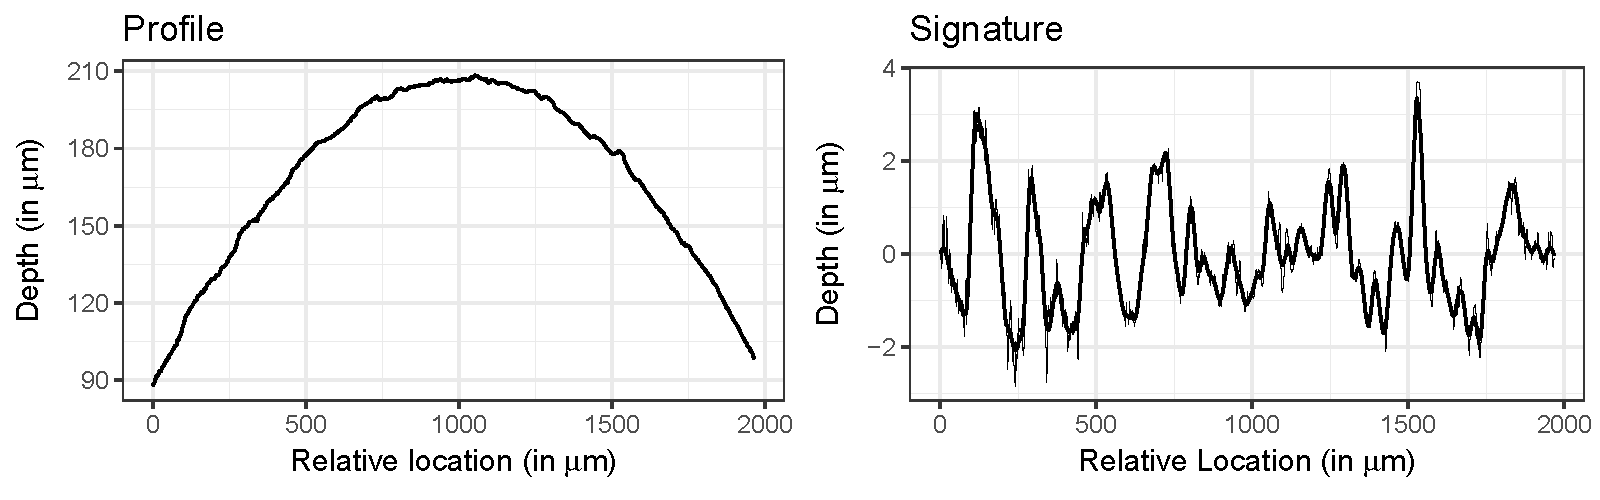
\includegraphics[width=\textwidth]{figures/sigs-profiles-1} 

}

\caption{Bullet land profile (left) and the corresponding signature (right) for one of the lands of Hamby-44.}\label{fig:sigs-profiles}
\end{figure}

In a pre-processing step the two markings are smoothed using a LOWESS
\citep{lowess} with coarseness parameter \(c\). Originally, this
smoothing is intended to remove drift and (sub)class characteristics
from individual markings, however, in the setting of matching bullet
striae, we can also make use of this mechanism to separate bullet
curvature in profiles from signatures before matching signatures.
\autoref{fig:sigs-profiles} shows an example of a bullet land profile
(left) and the corresponding signature (right).

After removing sub-class structure, the Chumbley score is calculated in
two steps: an optimization step and a validation step. In the
optimization step, the two markings are aligned horizontally such that
within a pre-defined window of length \(w_o\) the correlation between
\(x(t_1)\) and \(y(t_2)\) is maximized: \[
\left(t_1^o, t_2^o\right) = \mathop{\arg \max}\limits_{1 \le t_1 \le T_1-w_o, 1 \le t_2 \le T_2-w_o} \text{cor} \left(x^{w_o} (t_1), y^{w_o}(t_2) \right)
\] This results in an optimal vertical (in-phase) shift of
\(t_1^o - t_2^o\) for aligning the two markings. We will denote the
relative optimal locations as \(t_1^*\) and \(t_2^*\), where
\(t_i^* = t_i^o/(T_i-w_o)\) for \(i=1,2\), such that
\(t_1^*, t_2^* \in [0,1]\). Once (sub-)class characteristics are
removed, the relative optimal locations should be distributed according
to a uniform distribution in \([0,1]\).

In the validation step, two sets of windows of size \(w_v\) are chosen
from both markings, \autoref[see][]{fig:win-comparison}. In the first
set, pairs of windows are extracted from the two markings using the
optimal vertical shift as determined in the first step, whereas for the
second set the windows are extracted using a different (out-of-phase)
shift.

More precisely, let us define starting points \(s_i^{(k)}\) for each
signature \(k = 1, 2\) as

\begin{eqnarray}\label{eq.start}
s^{(k)}_i = 
\begin{cases}
t_k^* + i w_v & \text{ for } i < 0 \\
t_k^* + w_ o + i w_v & \text{ for } i \ge 0,
\end{cases}
\end{eqnarray}

for integer values of \(i\) with \(0 < s^{(k)}_i \le T_k - w_v\).

Same-shift pairs of length \(w_v\) are defined in \citet{hadler} as all
pairs \((s_i^{(1)}, s_i^{(2)})\) with integer values \(i\) for which
both \(s_i^{(1)}\) and \(s_i^{(2)}\) are defined. Similarly,
different-shift pairs are defined as \((s_i^{(1)}, s_{-i-1}^{(2)})\) for
all \(i\) where both \(s_i^{(1)}\) and \(s_{-i-1}^{(2)}\) are defined
(see \autoref{sketch-same-diff}).

\begin{figure}[hbtp]
\centering
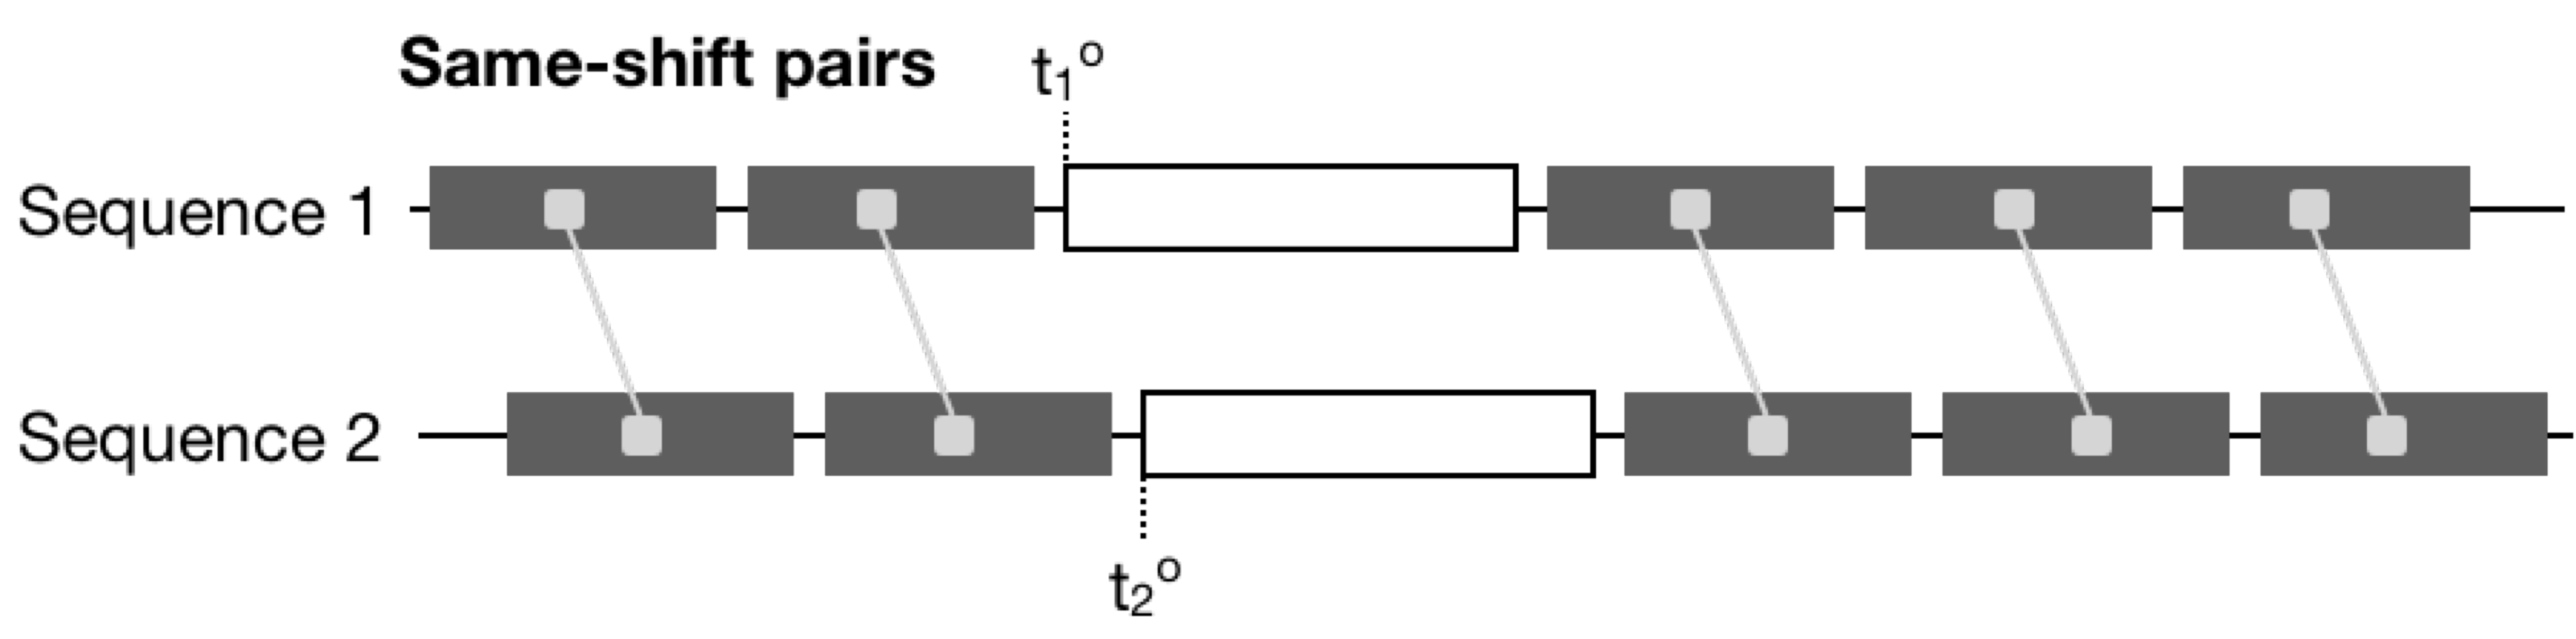
\includegraphics[width=.7\textwidth]{images/sketch-same.png}

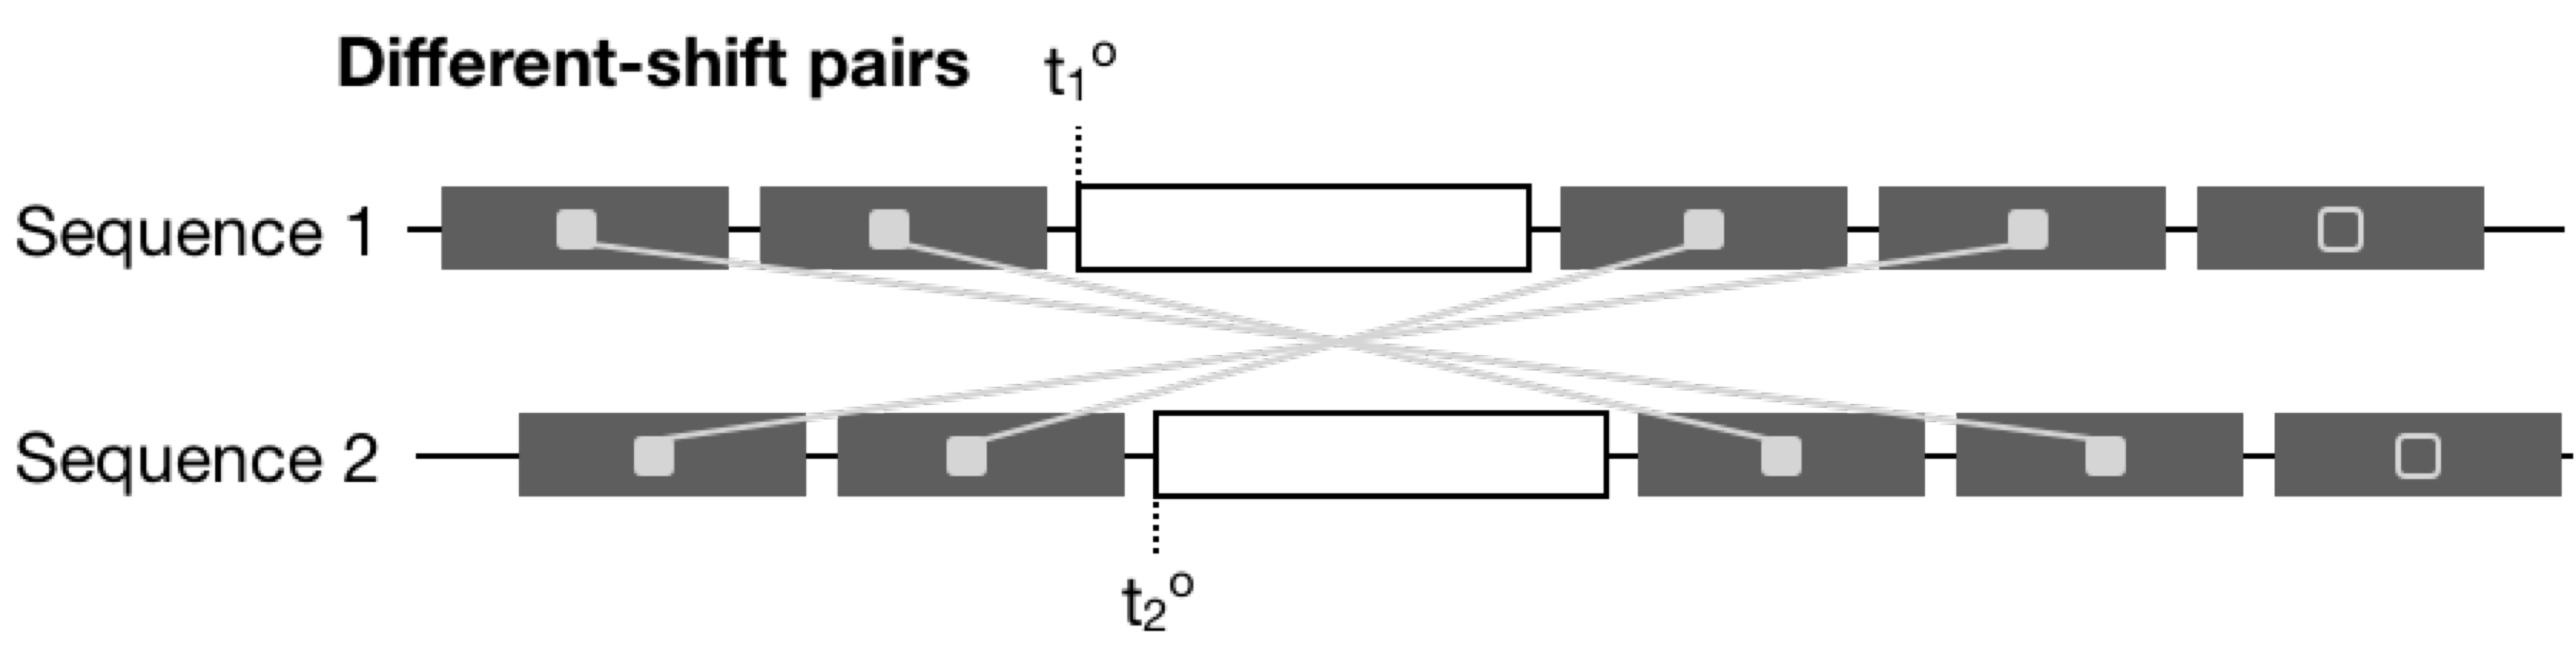
\includegraphics[width=.7\textwidth]{images/sketch-diff.png}
\caption{\label{sketch-same-diff}Sketch of same-shift pairings  (top) and different-shift pairings (bottom). Filled in rectangles show pairings resulting in correlations, unfilled rectangles are segments without a match.}
\end{figure}

\begin{figure}

{\centering 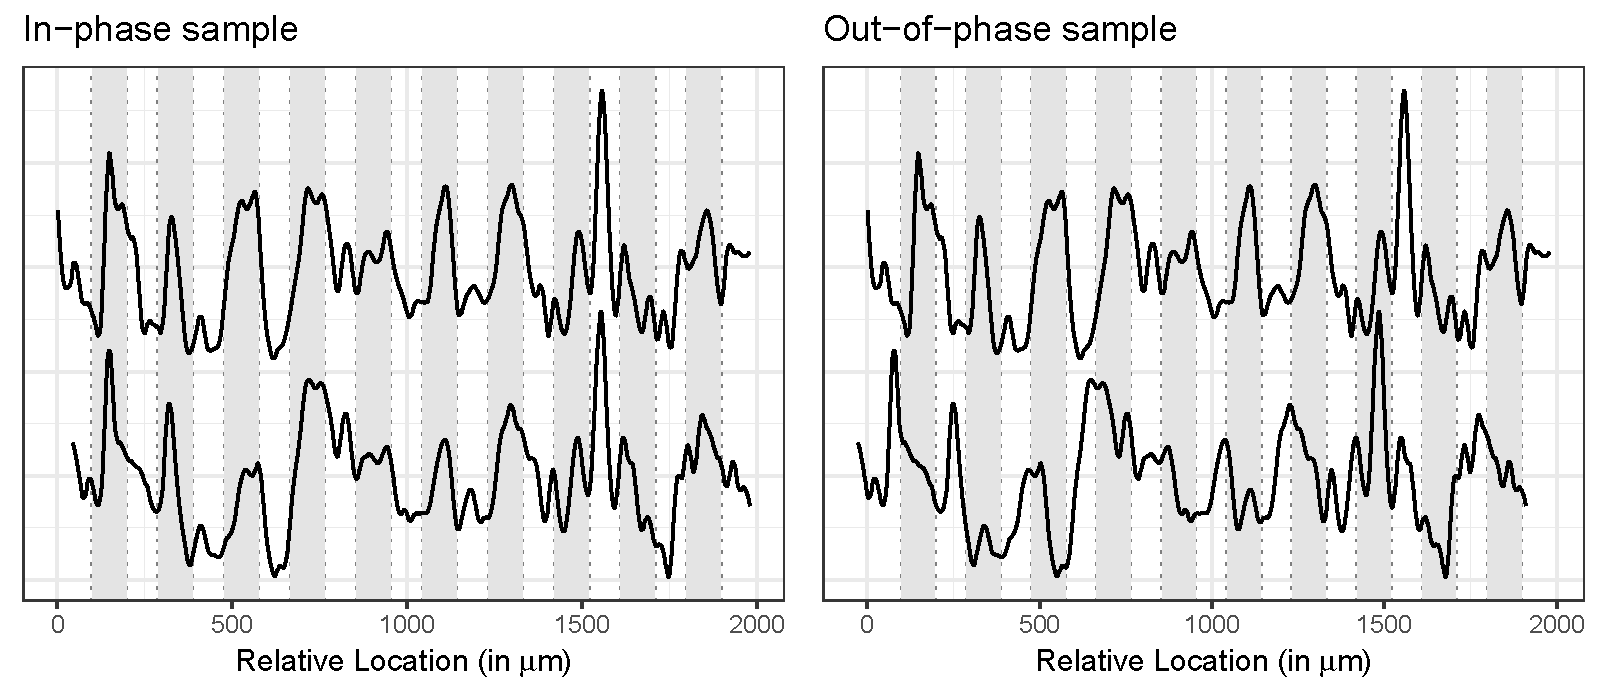
\includegraphics[width=\textwidth]{figures/win-comparison-1} 

}

\caption{Two same-source markings. For convenience, the markings are moved into phase on the left and out-of phase on the right. In-phase (left) and out-of-phase (right) samples are shown by the light grey background. The Chumbley-score is based on a Mann-Whitney U test of the correlations derived from these two sets of samples.}\label{fig:win-comparison}
\end{figure}

For both same- and different-shift pairs correlations between the
markings are calculated. The intuition here is that for two markings
from the same-source the correlation for the in-phase sample should be
high, while the correlations of the out-of-phase sample provide a
measure for the base-level correlation for non-matching marks of a given
length \(w_v\). The Chumbley score is then computed as a Mann Whitney U
statistic to compare between in-phase sample and out-of-phase sample. In
the original method proposed in \citet{chumbley} both in-phase and
out-of-phase sample are extracted randomly, whereas \citet{hadler}
proposed the above specified deterministic rules for both samples to
make the resulting score deterministic while simultaneously avoiding
overlaps within selected marks to ensure independence.

\subsection{A problem with failed
tests}\label{a-problem-with-failed-tests}

Looking closer at \autoref{eq.start}, we see that by definition, some
number of tests will fail to produce a result. The problem of failed
tests is first mentioned in \citet{afte-chumbley}. Unfortunately, the
authors do not provide any percentage of how many tests failed for their
data. The algorithm fails to produce for two reasons: either the number
of eligible same-shift pairs is zero, or the number of different-shift
pairs is zero.

The number of same-shift pairs will be zero, if the optimal locations
\(t_1^{o}\) and \(t_2^{o}\) are so far apart, that no segments of size
\(w_v\) are left on the same sides of the optimal locations, i.e.
\(t_1^{o} < w_v\) and \(t_2^{o} > T_2-w_o-w_v\) or
\(t_1^{o} < T_1- w_o - w_v\) and \(t_2^{o} < w_v\), i.e.~we have a
failure rate of \[
P\left( t_1^{o} < w_v \ \cap \ t_2^{o} > T_2-w_o-w_v\right) + P\left( t_1^{o} < T_1- w_o - w_v \ \cap \ t_2^{o} < w_v\right).
\] While we can assume that once (sub-)class characteristics are
removed, optimal locations \(t_i^{o}\) are uniformly distributed across
the length of the profile, we cannot assume that \(t_1^o\) and \(t_2^o\)
are independent of each other. In particular, for same-source profiles,
we would expect a strong dependency between these locations, in which
case a large difference between locations is unlikely. However, for
different-source matches, we can assume that locations are independent.
In that case, we expect a test to fail with a probability of
\(\frac{2 w_v^2}{(T_1-w_o)(T_2-w_o)}\). For an average length of \(T_i\)
of 1200 pixels, \(w_o = 120\) pixels and \(w_v = 30\) pixels this
probability is about 0.0015.

The number of possible different-shift pairs also depends on the
location of the optimal locations \(t_1^o\) and \(t_2^o\). Whenever the
optimal locations are close to the boundaries, the number of possible
pairings decreases and reaches zero, if \(t_i^{(o)} < w_v\) or
\(t_i^{(o)} > T_i-w_o- w_v\). Assuming a correlation between optimal
locations \(t_1^o\) and \(t_2^o\) of close to one for same-source
profiles, this results in an expected rate of failure of
\(2 w_v / (T_i-w_o)\), or about 5.6\% for an average length of \(T_i\)
of 1200 pixels, \(w_o = 120\) pixels and \(w_v = 30\) pixels. Assuming
independence in the optimal locations for different-source profiles the
expected probability for a failed test is, again,
\(\frac{2 w_v^2}{(T_1-w_o)(T_2-w_o)}\).

\subsection{A modified approach}\label{a-modified-approach}

While failures due to missing correlations from same-shift pairs are
unavoidable by definition of the Chumbley score, failures due to missing
correlations from different-shift pairs can be prevented by using a
different strategy in assigning pairs.

Using the same notation as in \autoref{eq.start}, we define same-shift
pairs identical to \citet{hadler} as pairs \((s_i^{(1)}, s_i^{(2)})\)
for all \(i\) where the boundary conditions of both sequences are met
simultaneously. Let us assume that this results in \(I\) pairs. Define
\(s_{(j)}^{(k)}\) to be the \(j\)th starting location in sequence
\(k = 1, 2\),
i.e.~\(s_{(1)}^{(k)} < s_{(2)}^{(k)} < ... < s_{(I)}^{(k)}\).

We then define the pairs for different-shifts as

\begin{equation}\label{eq.diff2}
\left(s_{(j)}^{(1)}, s_{(I-j+1)}^{(1)} \right) \text{ for } j = 
\begin{cases}
1, ..., I & \text{ for even } I \\
1, ..., (I-1)/2, (I-1)/2 + 2, ..., I & \text{ for odd } I
\end{cases},
\end{equation}

i.e.~for an odd number of same-shift correlations, we skip the middle
pair for the different-shift correlations (see \autoref{sketch-diff-2}).
This pairing ensures that the number of different-shift pairings is the
same or at most one less than the number of same-shift pairings in all
tests. In the remainder of the paper, we will refer to the algorithm
defined by \citet{hadler} as \textbf{(CS1)} and the suggested modified
algorithm as \textbf{(CS2)} and compare their performance on the
available scans of the Hamby study. The section  A %\ref{appendix:appxfailed} 
of the Appendix discusses about the various scenarious of failed tests.

\begin{figure}[hbtp]
\centering
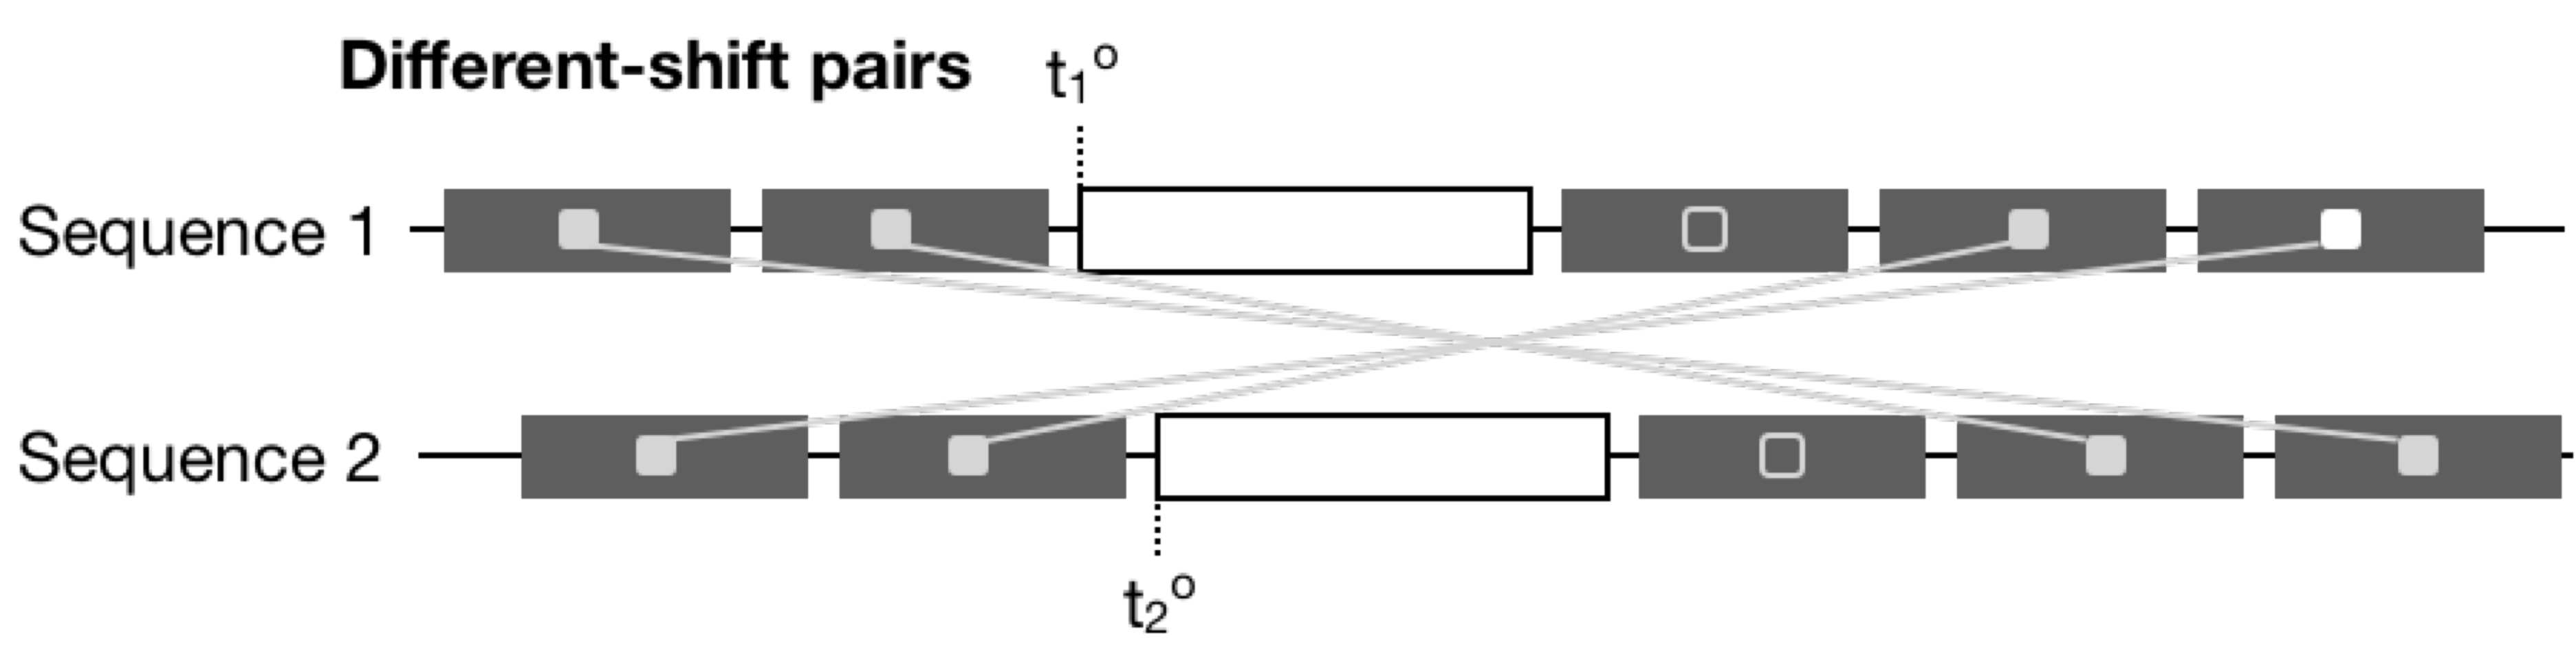
\includegraphics[width=.7\textwidth]{images/sketch-diff-2.png}
\caption{\label{sketch-diff-2}Sketch of adjusted different-shift pairings. At most one of the same-shift pairings can not be matched with a different-shift pair under algorithm (CS2). }
\end{figure}

\subsection{Testing setup}\label{testing-setup}

\subsubsection{The Data}\label{the-data}

Lands for all Hamby-44 and Hamby-252 scans are made available through
the NIST ballistics database \citep{nist} and are considered, here. Both
of these sets of scans are part of the larger Hamby study \citep{hamby}.
Each set consists of twenty known bullets (two each from ten
consecutively rifled Ruger P85 barrels) and fifteen questioned bullets
(each matching one of the ten barrels). Ground truth for both of these
Hamby sets is known and was used to assess correctness of the tests
results.

Profiles for each bullet land were extracted from scans close to the
heel of the bullet while avoiding break-off as described in
\citet{aoas}.

\subsubsection{Setup}\label{setup}

Both algorithms (CS1) and (CS2) are implemented in R \citep{R}. (CS1) is
available from package \texttt{toolmaRk} \citep{toolmark}, (CS2) is
available from a modified version of the \texttt{toolmaRk} package
available from GitHub (\url{https://github.com/heike/toolmaRk}). We
applied both methods to all pairwise land-to-land comparisons of the
Hamby scans provided by NIST for a total of 85,491 land-to-land
comparisons.

\section{Results}\label{results}

\subsection{Failed Tests}\label{failed-tests}

As described above, the Chumbley-score is based on three parameters:
coarseness \(c\) and the sizes of the optimization window \(w_o\) and
validation window \(w_v\). In a first run of results, we applied default
settings for the parameters, as suggested in \citet{hadler}:
\(w_o = 120\) pixels or about 190 \(\mu m\) (ten percent of the average
length of profiles) and coarseness \(c = 0.25\), and varied the size of
the validation window \(w_v\) in steps of 10 from 10 pixels to 60
pixels. Based on a significance level \(\alpha\) of 0.05 for the test,
this results in a correct identification of same-source and
different-source toolmarks of 93.5\% to 94.1\%, corresponding to a rate
of false negatives between 0.28 and 0.36 and a rate of false positives
between 0.05 and 0.06. However, the most prominent result we
encountered, are the high number of failed tests, i.e.~the number of
instances, in which CS1 did not return any result. \autoref{fig:fails}
shows the percentage of failed tests among the 85,491 land-to-land
comparisons of the NIST data for different values of the validation
window size \(w_v\). For same-source lands up to 12.5 percent of the
tests fail using CS1. The highest percentage of failed tests under CS2
is 1.3\% for different-source tests using a validation window size
\(w_v\) of 60 pixels. Rates of expected failures are based on simulation
runs using covariances between locations of same-source profiles of
0.854, and 0.120 for locations from different-source profiles, matching
observed covariances for the Hamby scans. Observed failure rates are
higher than expected. This might be due to remaining sub-class structure
at a coarseness of 0.25 resulting in a distribution of optimal locations
different from the assumed uniform.

\begin{figure}

{\centering 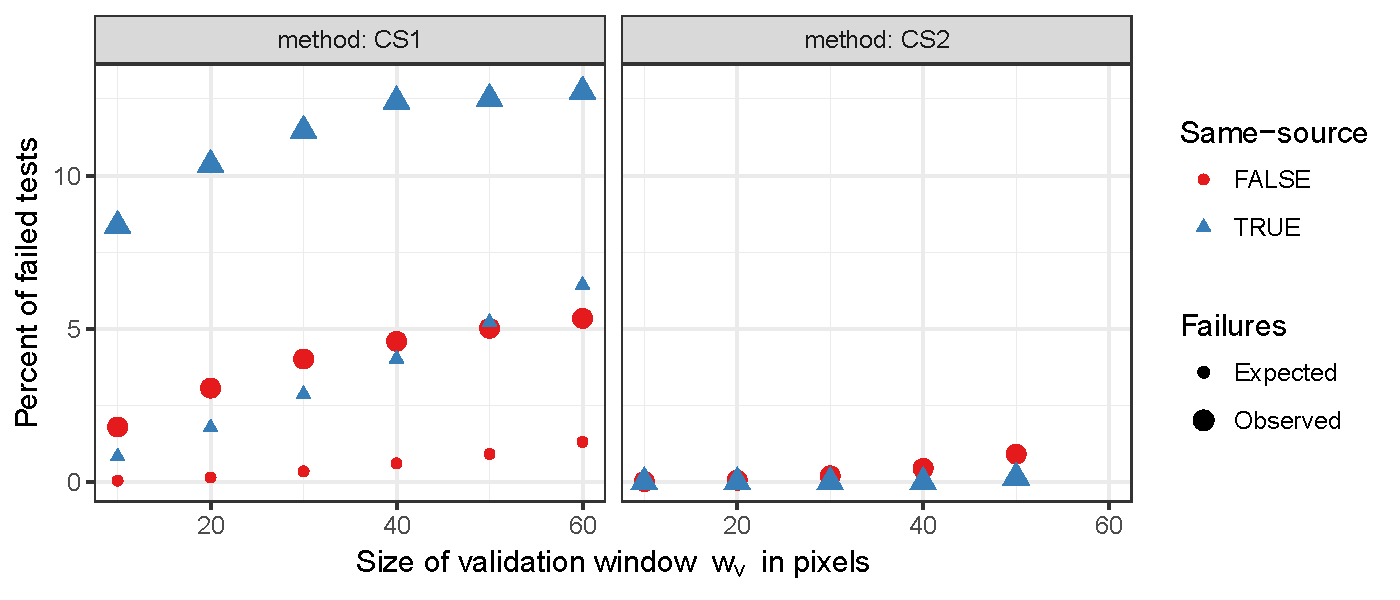
\includegraphics[width=0.7\textwidth]{figures/fails-1} 

}

\caption{Percent of failed land-to-land comparisons using an optimization window $w_o = 120$ and a coarseness of $c = 0.25$. With an increase in the size of the validation window  a higher percentage of tests fails under both methods (CS1) and (CS2), but the percentage of failed tests is much smaller under (CS2). Observed failure rates of (CS1) are higher than expected rates.}\label{fig:fails}
\end{figure}

\subsection{Coarseness}\label{coarseness}

The purpose of the coarseness parameter is to remove (sub-)class
characteristics from profiles before comparisons for matching.
\citet{hadler} suggest a coarseness parameter of 0.25 in the setting of
toolmark comparisons. For bullet lands, coarseness might need to be
adjusted because of the strong effect bullet curvature has on profiles.

\autoref{fig:profile-sketch} gives an overview of the effect of
different coarseness parameters: from left to right, coarseness levels
\(c\) are varied in steps of 0.05 from 0.1 to 0.3. The top row shows
resulting signatures after smoothing the profile shown in
\autoref{fig:sigs-profiles} with different levels of coarseness. The
histograms in the bottom row show the relative optimal location \(t^*\).
Optimal locations are distributed uniformly once (sub-)class
characteristics are removed. However, for coarseness values of
\(c > 0.20\) we see quite distinct boundary effects: optimal locations
\(t^*\) are found at the very extreme ends of a profile more often than
one would expect based on a uniform distribution.

The key effect of the optimal locations and thereby the coarseness is
seen in the number of failed tests. Irrespective of whether CS1 or CS2
is being used, if the relative optimal locations are at the boundaries
we will see an increase in the number of failed tests. A balance is
therefore needed in the selection of the coarseness parameter which
reduces the boundary effect but does not remove important individual
characteristics. Based on \autoref{fig:profile-sketch} a coarseness
value of \(c = 0.15\) seems to be best suited to strike this balance for
this example. For the remainder of the analysis, we will use this value
for \(c\).

\begin{figure}

{\centering 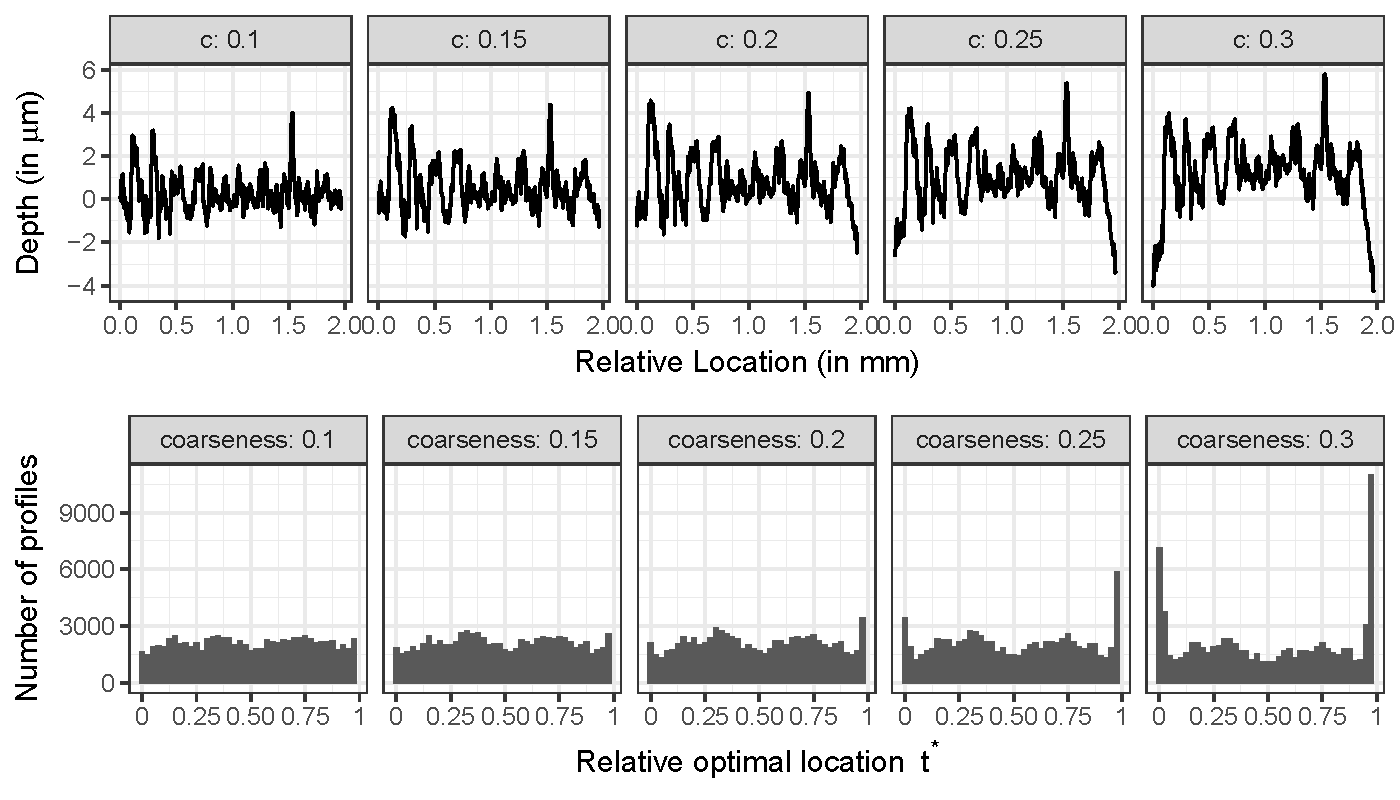
\includegraphics[width=\textwidth]{figures/profile-sketch-1} 

}

\caption{Overview of the effect of different coarseness parameters $c$ on the profile shown in Figure \ref{fig:sigs-profiles} (top). The bottom row shows histograms of  the (relative) optimal locations $t^o$ identified in the optimization step for different values of the coarseness parameter $c$. }\label{fig:profile-sketch}
\end{figure}

\subsection{Error rate assessment}\label{error-rate-assessment}

\autoref{fig:roc} gives an overview of ROC (Receiver operating
characteristic) curves for methods CS1 and CS2 over a range of different
optimization window sizes \(w_o\) and two sizes for the validation
window \(w_v\) (shape). The different color hues represent the two
methods CS1 (red) and CS2 (blue). The ROC curves show the superior
performance of CS2 over CS1. Generally, an optimization window \(w_o\)
of 150 pixels or more leads to the best performance with respect to ROC
curves. Results based on a validation window of size \(w_v = 30\) are
generally better than results for \(w_v = 50\).

\autoref{fig:eer} shows a comparison of the performance of the two
methods CS1 and CS2 with respect to EER (equal error rate) and AUC (area
under the curve) corresponding to the ROC curves shown in
\autoref{fig:roc}. Equal error rates are reduced using method CS2, while
area under the curve significantly increases (at a significance level
\(\alpha\) of 0.05) compared to method CS1.

The results from Figures \ref{fig:roc} and \ref{fig:eer} are summarized
in numbers in \autoref{tab:aucs}. Equal error rates (EER), rates for
false positives (FPR) and false negatives (FNR) are shown side by side
with the area under the curve (AUR) for both methods for a set of
different optimization windows \(w_o\) and a validation window \(w_v\)
of 30 pixels. The rate of false positive same-source identifications is
equal to the statistical type I error rate, which is set to
\(\alpha = 0.05\) for this example. The rate of false negatives are
missed same-source markings. This rate is also known as the type II
error rate. A detailed plot on the type II error rates for CS1 and CS2 
can be found in the section B %\ref{appendix:appxtype2} 
of the Appendix.\\
Area under the curve (AUC) is shown with confidence intervals as given
by \citet{delong}. CS2 significantly outperforms CS1 with respect to its
predictive power in most situations.

\begin{figure}

{\centering 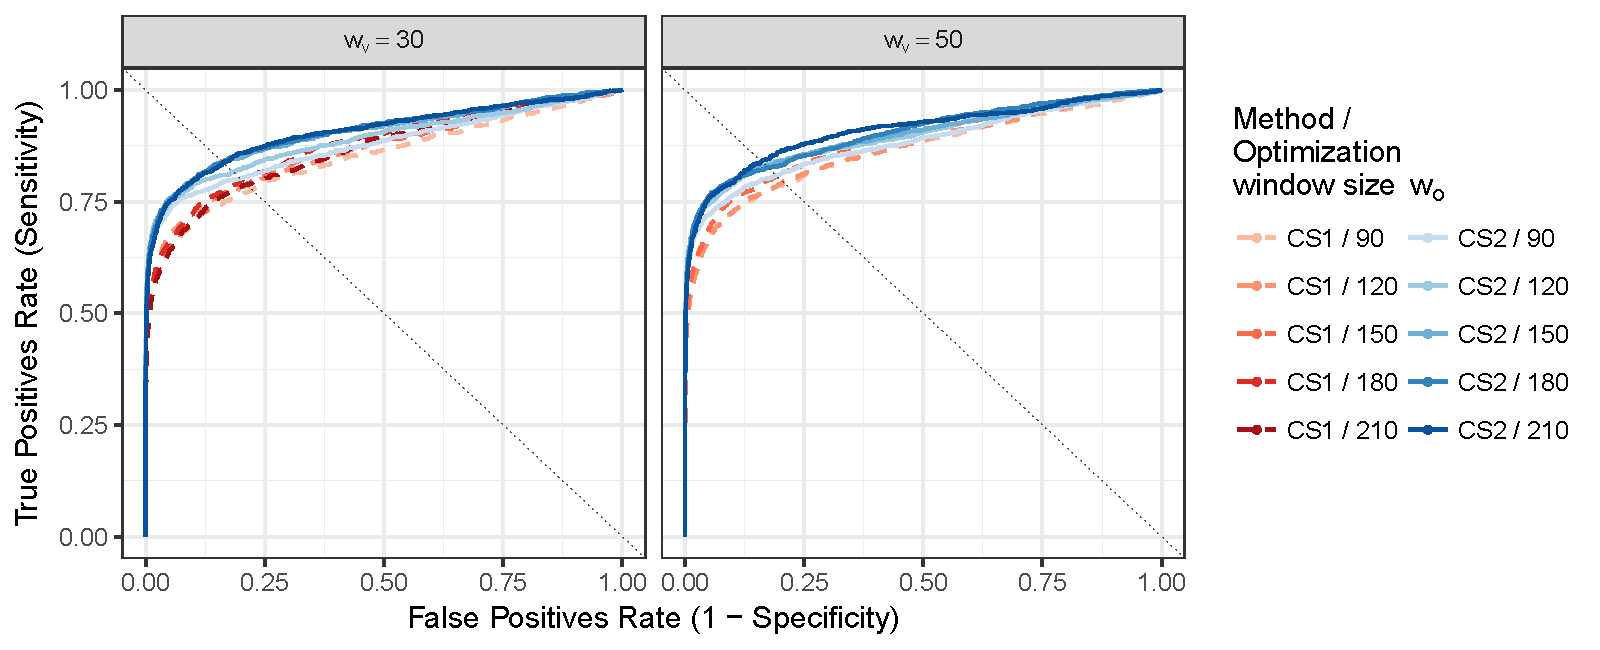
\includegraphics[width=\textwidth]{figures/roc-1} 

}

\caption{ROC curves of methods CS1 and CS2 for different sizes of optimization window $w_o$. Best performances with respect to  ROC curves are reached for optimization windows of sizes 150 and higher. Points of equal error rates (EERs) can be found at the intersection of the dotted line and the ROC curves.}\label{fig:roc}
\end{figure}

\begin{figure}

{\centering 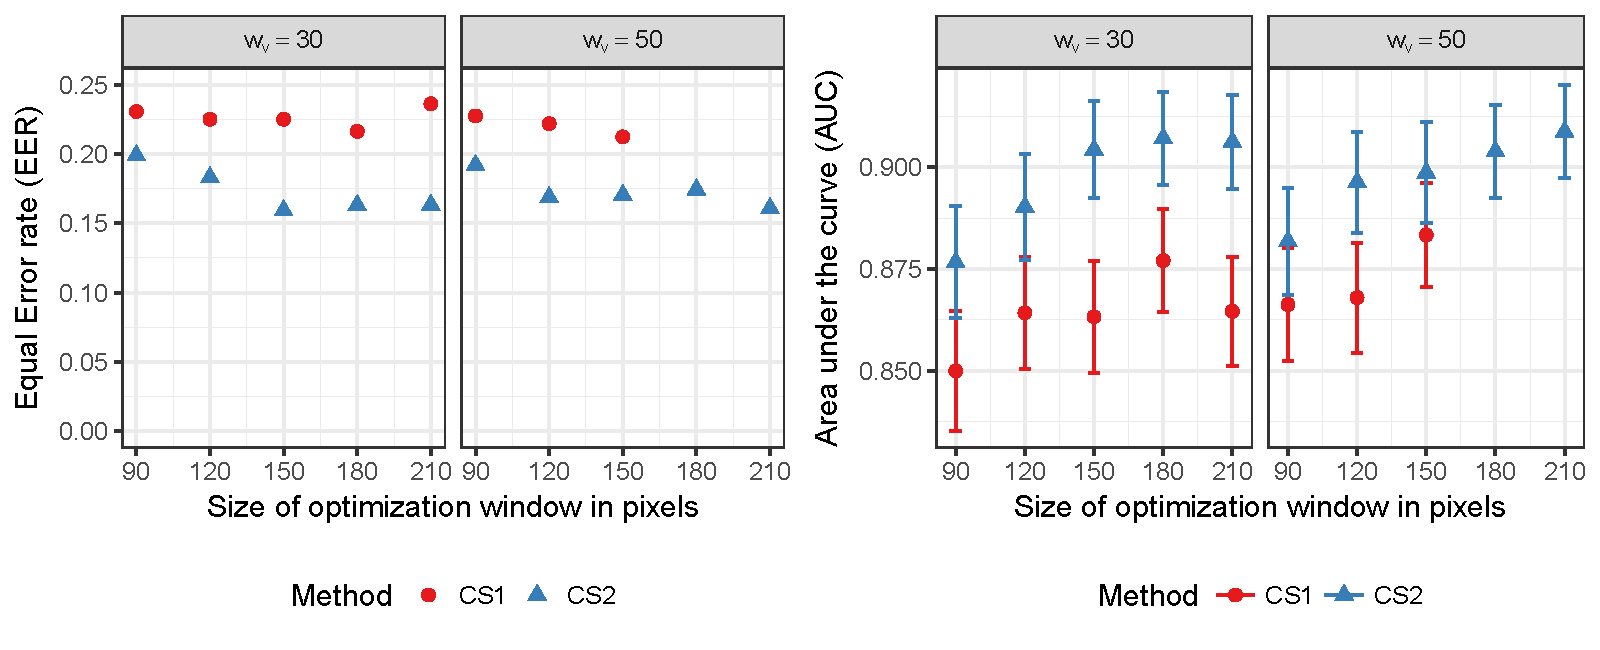
\includegraphics[width=\textwidth]{figures/eer-1} 

}

\caption{Comparison of results for CS1 and CS2 using area under the curve (AUC) and equal error rates (EER). }\label{fig:eer}
\end{figure}

\begin{table}[hbtp]
\centering
\begin{adjustbox}{max width=\textwidth}
\begin{tabular}{rrrlrrl}
  \hline
  & \multicolumn{3}{l}{\bf CS1} & \multicolumn{3}{l}{\bf CS2} \\
$w_o$ & \bf FPR & \bf FNR & \bf AUC (95\% C.I.) & \bf FPR & \bf FNR & \bf AUC (95\% C.I.) \\ 
  \hline
90 & 0.068 & 0.330 & 0.850 (0.835, 0.865) & 0.075 & 0.242 & 0.877 (0.863, 0.890) \\ 
  120 & 0.065 & 0.309 & 0.864 (0.850, 0.878) & 0.072 & 0.236 & 0.890 (0.877, 0.903) \\ 
  130 & 0.065 & 0.317 & 0.863 (0.850, 0.877) & 0.072 & 0.224 & 0.898 (0.886, 0.910) \\ 
  140 & 0.065 & 0.304 & 0.873 (0.859, 0.886) & 0.071 & 0.229 & 0.902 (0.891, 0.914) \\ 
  150 & 0.067 & 0.326 & 0.863 (0.850, 0.877) & 0.072 & 0.225 & 0.904 (0.892, 0.916) \\ 
  180 & 0.061 & 0.326 & 0.877 (0.864, 0.890) & 0.070 & 0.229 & 0.907 (0.896, 0.919) \\ 
  210 & 0.064 & 0.342 & 0.865 (0.851, 0.878) & 0.066 & 0.231 & 0.906 (0.895, 0.918) \\ 
   \hline
\end{tabular}
\end{adjustbox}
\caption{\label{tab:aucs} Overview of results as shown in Figures \ref{fig:roc} and \ref{fig:eer}. FPR is the observed rate of false positives (for a fixed level $\alpha = 0.05$), FNR is the false negative rate. Area under the curve (AUC) is shown with confidence intervals. }
\end{table}

\subsection{Observed versus Nominal Type I error
rates}\label{observed-versus-nominal-type-i-error-rates}

\autoref{fig:type1} shows observed type I error rates (FPR) across a
range of optimization windows \(w_o\). Generally, observed type I errors
are higher than expected. Method CS1 shows in this instance slightly
better performance than method CS2, but for both an increase in the size
of the optimization window leads to a decrease in the observed type I
error rates.

\begin{figure}

{\centering \includegraphics[width=\textwidth]{figures/type1-1} 

}

\caption{Comparison of observed and nominal type I error rates  across a range of window sizes for optimization $wo$. The horizontal line in each facet indicates the nominal type I error rate.}\label{fig:type1}
\end{figure}

\subsection{High resolution Hamby 44
scans}\label{high-resolution-hamby-44-scans}

The high-resolution scans of Hamby set 44 are capturing images at a
resolution of \(0.645 \mu m\) per pixel. On average, land engraved areas
are 3000 pixels in length. A coarseness of \(c = 0.125\) seemed to be
sufficient in removing any bullet curvature. Both methods have a failed
test rate of less than 0.006, indicating, again, that the larger number
of pixels alleviates the problem of test failures. \autoref{fig:h44}
shows the resulting EER and AUC for methods CS1 and CS2 based on two
sizes of validation windows (\(w_v \in 75, 125\)) and optimization
window sizes around 300 pixels (10 percent of the average length). Both
methods show an increase in performance around \(w_o = 300\) pixels. CS2
out-performs CS1 in all scenarios, but the difference is not significant
(using DeLong's confidence intervals). Interestingly, the overall
performance of both CS1 and CS2 is a lot lower for the high resolution
version of Hamby-44 than for the lower resolution scans. The area under
the curve overall is significantly lower for the high resolution scans
than for the previous set of scans. Partly, this might be due to the
particular choice of the parameters, partly the higher-resolution scans
might be picking up on real differences between the lands that the
lower-resolution scans fail to detect.

\begin{figure}

{\centering \includegraphics[width=\textwidth]{figures/h44-1} 

}

\caption{AUC and EER for methods CS1 and CS2 based on high resolution scans of Hamby 44. }\label{fig:h44}
\end{figure}

\section{Conclusions}\label{conclusions}

In assessing the suitability of the (deterministic) Chumbley Score for
matching striae on bullet lands we have gained valuable insights into
the process: method CS1 as proposed by \citet{hadler} has a strong
dependency on the specific choice of parameters; the defaults suggested
by \citet{hadler} for screw drivers are not directly applicable for the
smaller bullet lands. The coarseness parameter in particular has a
strong impact on the performance of the test. However, we were able to
suggest some heuristics based on the assumption that once sub-class
characteristics are removed, optimal locations are distributed uniformly
across the profile. For bullet lands we found a coarseness value of
\(c = 0.15\) to be suitable for the low-resolution scans from NIST and a
value of \(c=0.125\) suitable for the higher-resolution scans from
CSAFE. Sizes for optimization windows \(w_o\) were based on
cross-validation to minimize overall type 2 error rates. Unfortunately,
this kind of assessment is only feasible in the setting of a large
study, such as the one we presented, and does not transfer immediately
to case work, where a forensic examiner would only deal with a few
identifications. Parameter settings for different studies should be
investigated and reported to allow for a further refinement.

Method CS1 proposed by \citet{hadler} has a minimal type 2 error rate of
0.272 for an optimized window size of 140 pixels -- which is
considerably higher than the error rates achieved on matching toolmarks,
but is similar to other single-feature methods proposed for bullet
matching. Unfortunately, method CS1 also has a high rate of failed tests
-- situations, in which the algorithm does not provide a result, due to
the way different-shift pairs are constructed. Algorithm CS2 is
introduced here as a remedy for failed tests by introducing an alternate
version of choosing different-shift pairs. The algorithm CS2 introduced
here is constructed in a way that achieves on average a ten-fold
reduction in the number of failures. While reducing the failure rate,
the algorithm also shows an increase in the power of the test. Type II
error rates of CS2 reach a minimum of 0.217 for an optimized window size
of 130 pixels. This increase in power of CS2 over CS1 should also apply
to previous studies on toolmarks. It would be interesting to see these
results using the adjusted algorithm. Unfortunately, none of the studies
have made the data publicly accessible.

While significantly reduced over CS1, CS2 still has type 2 error rates
on bullet lands that are higher than the error rates achieved on the
--much larger-- toolmarks. Applying these methods to the high-resolution
scans provided by CSAFE shows that better scanning methodology does not
guarantee a better matching performance.

However, bullets usually have multiple lands -- in the case of Ruger
P85s as used in the Hamby study, there are six lands for each bullet. We
might be able to get more power out of the test by adapting CS2 to work
in a bullet-to-bullet comparison.

\begin{comment}
\section{Appendix}\label{appendix}

\begin{appendix}

\section{Scenarios of failed tests}
\label{appendix:appxfailed}
Figures \ref{same-shift-failure} and \ref{diff-shift-failure} show scenarios in which the deterministic Chumbley score can fail. 
In \autoref{same-shift-failure} both CS1 and CS2 fail, because the lag between optimal locations is so large that no same-shift pairs can be found once the signatures are aligned. These failures are inherent to the Chumbley Score and cannot be prevented.
\begin{figure}[hbtp]
\centering
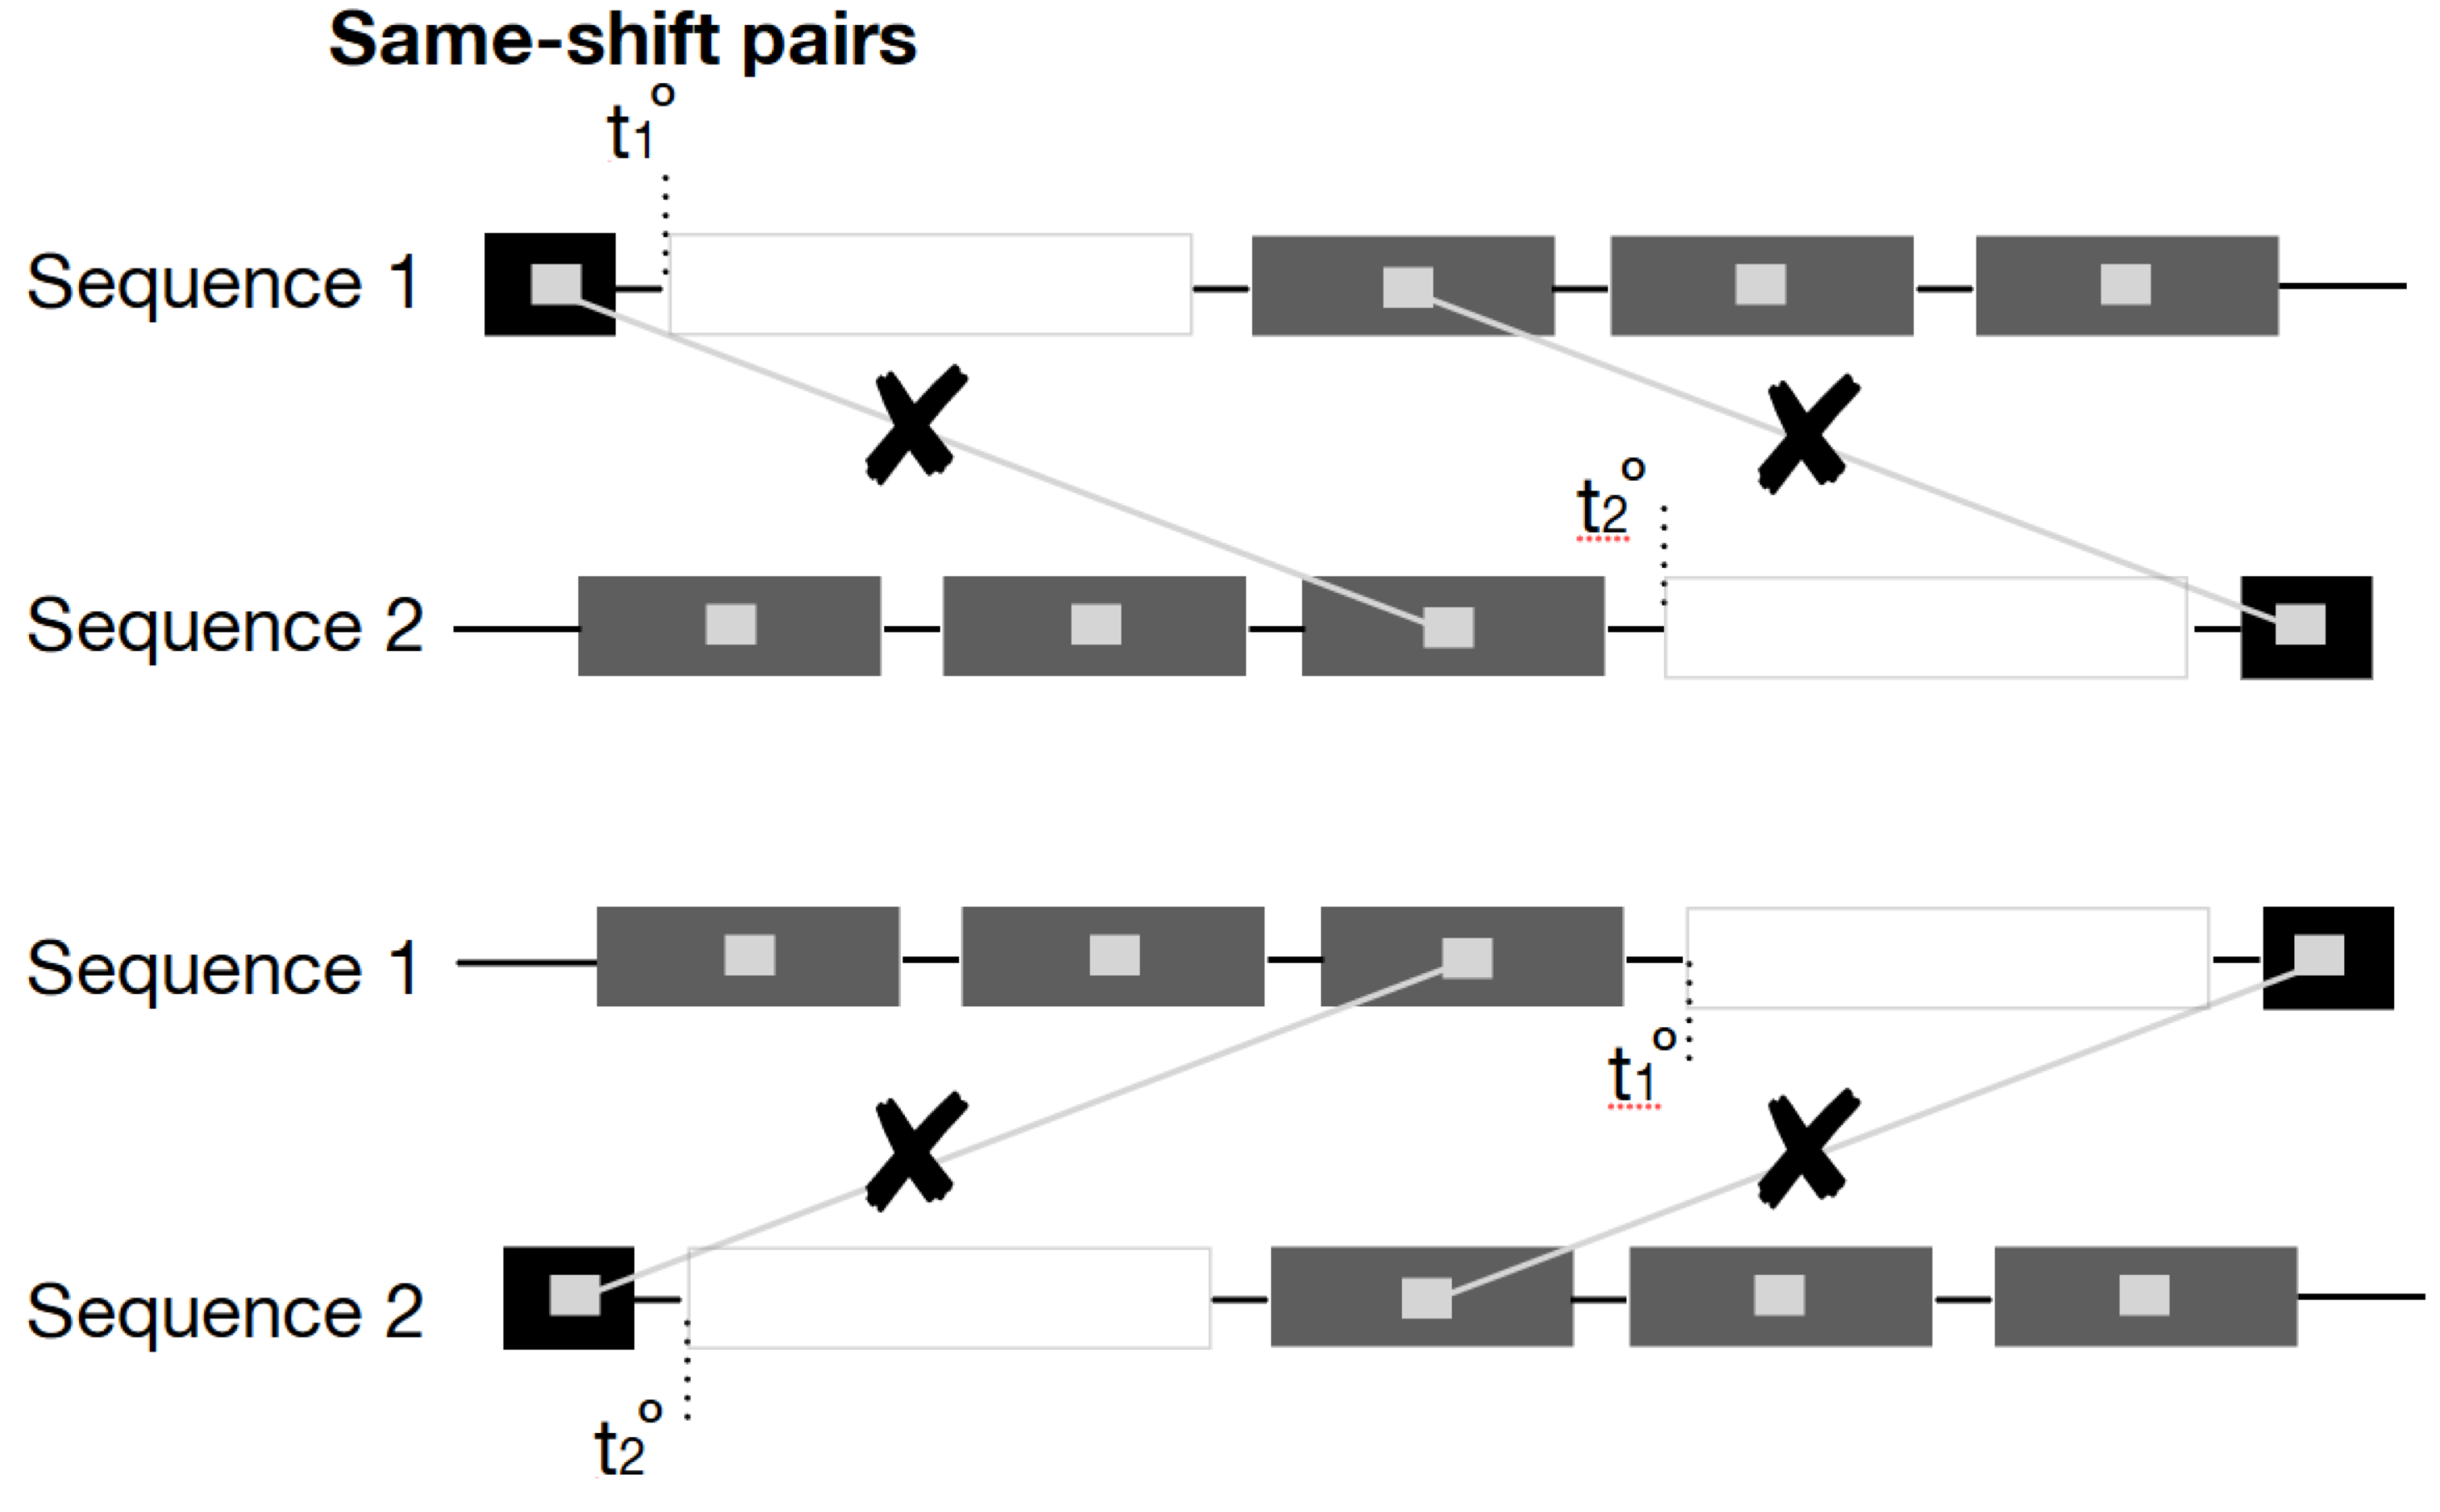
\includegraphics[width=0.62\textwidth]{images/same-shift-failure.png}

\caption{\label{same-shift-failure}Sketch of same-shift pairings. When the lag between optimal reference points is too large to accommodate a validation window in both signatures, both CS1 and CS2 fail.}
\end{figure}

\autoref{diff-shift-failure} shows two situations, in which CS1 fails to identify any different-shift pairings. This happens, when both relative locations are close to either end of the signature. CS2 can still be computed in this situation as long as there are at least two same-shift pairs identified. 

\begin{figure}[hbtp]
\centering
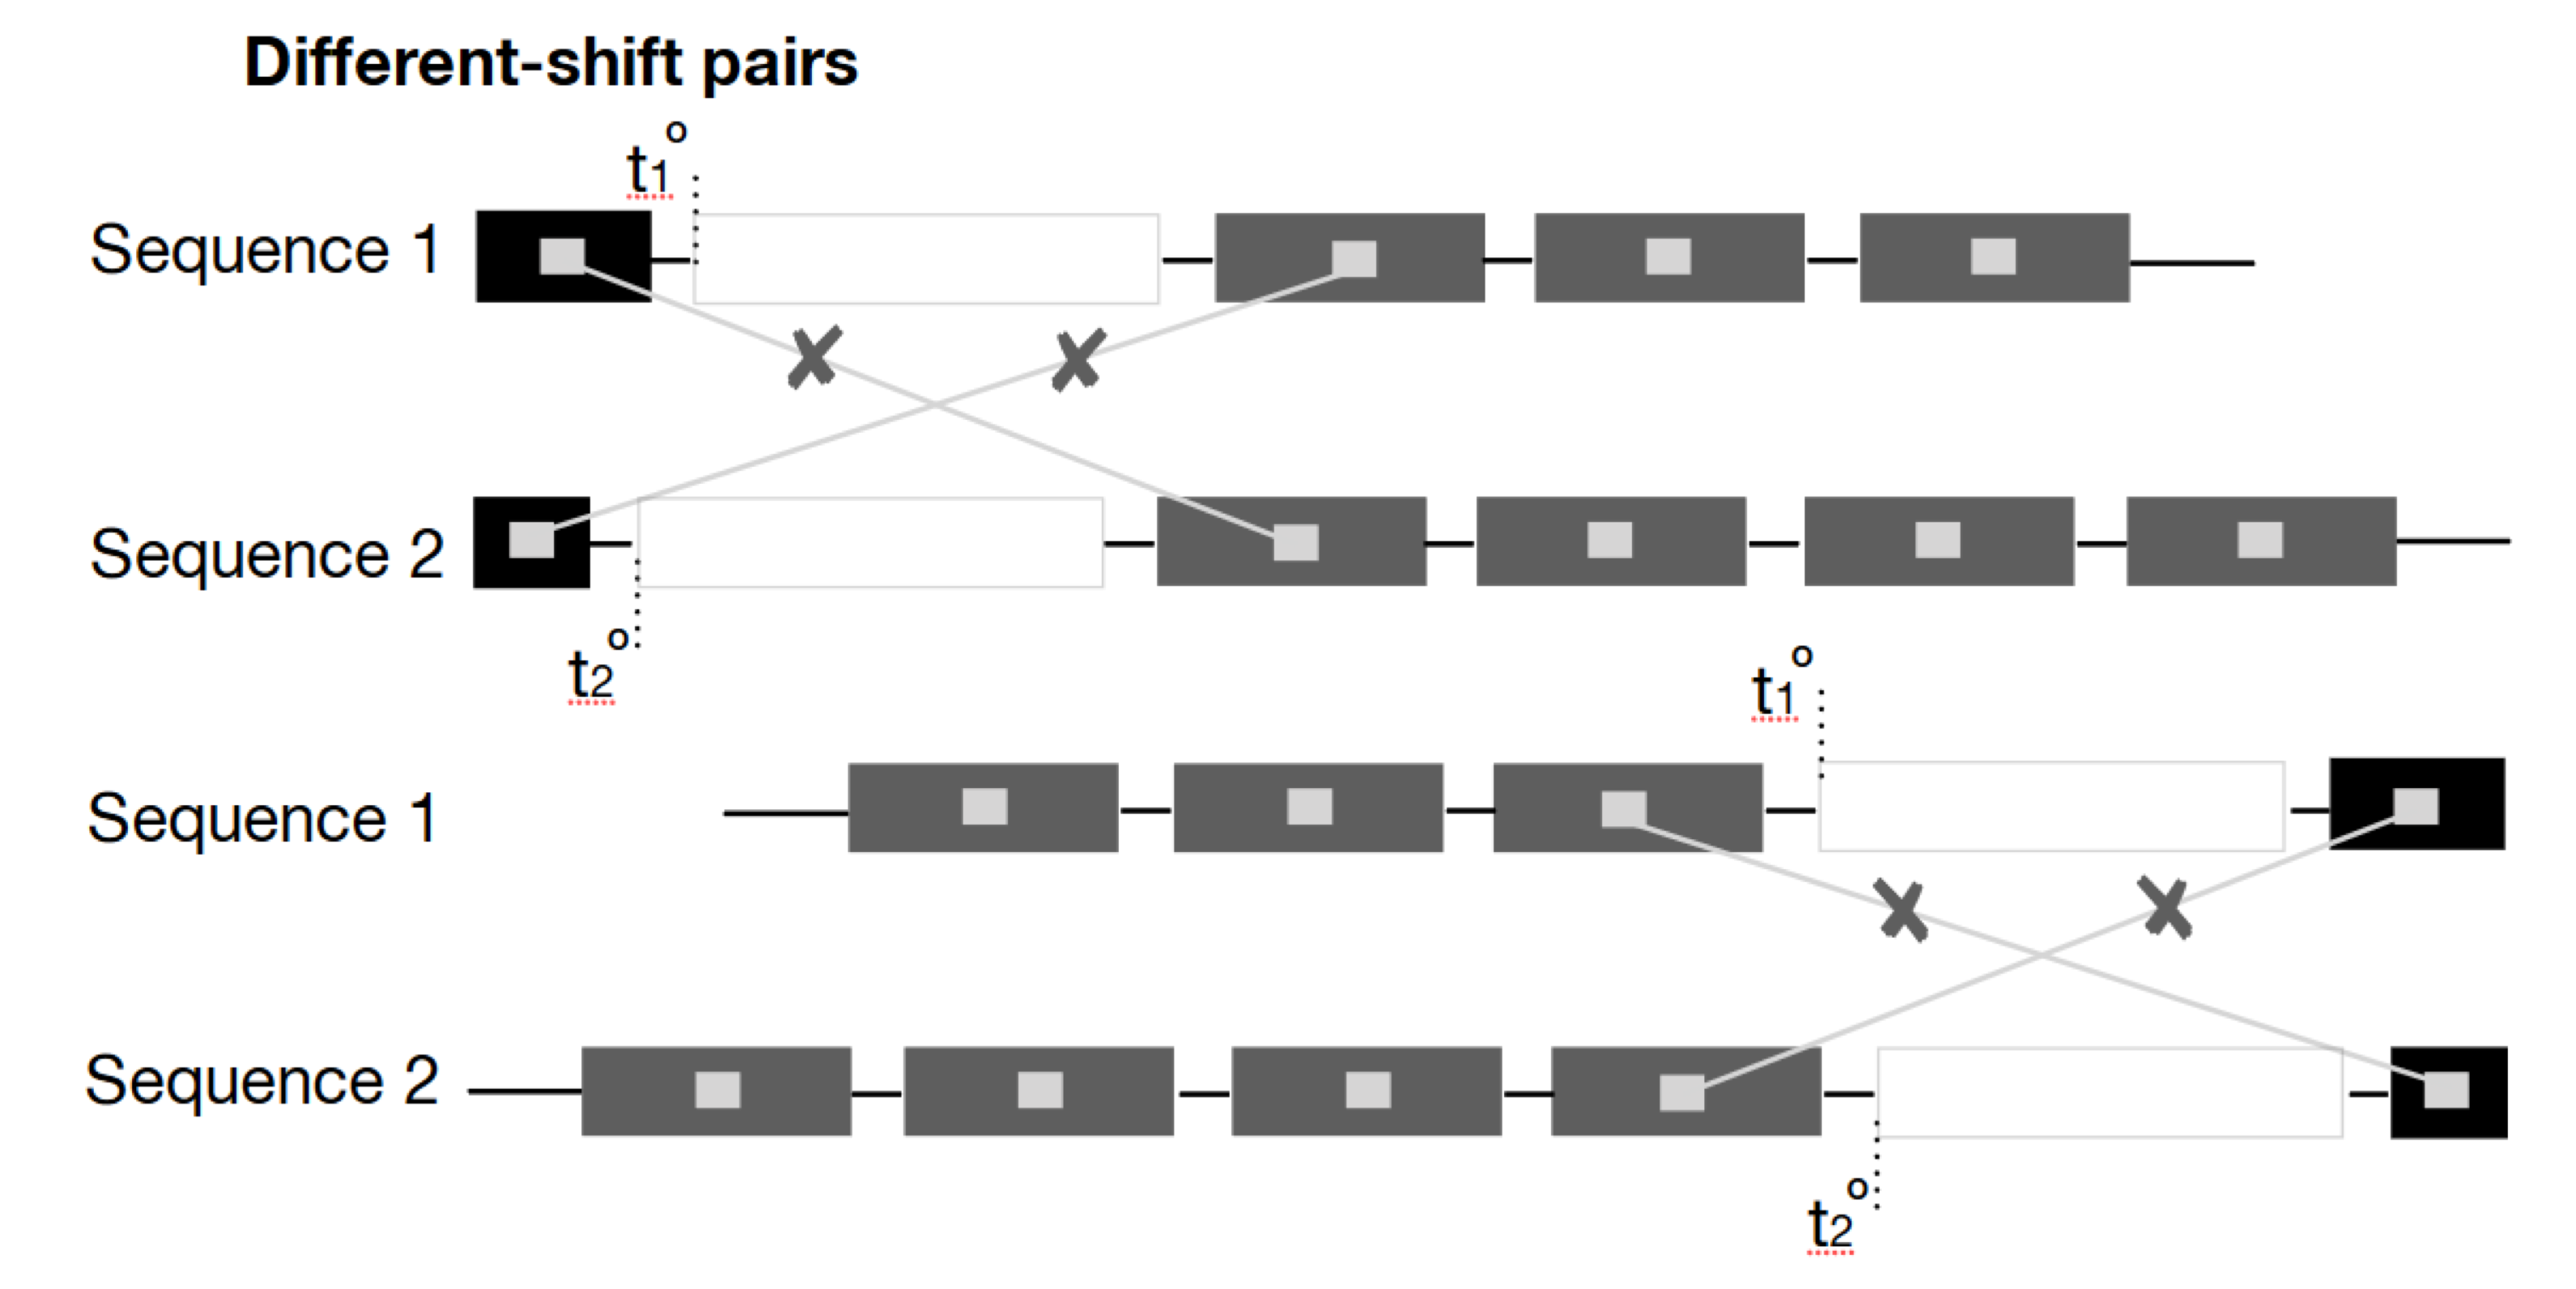
\includegraphics[width=0.7\textwidth]{images/diff-shift-failure.png}

\caption{\label{diff-shift-failure}Sketch of different-shift pairings. For CS1 no different-shift pairs can be identified, resulting in a failed test.}
\end{figure}

\newpage
\section{Type 2 errors: CS1 vs CS2}
\label{appendix:appxtype2}
\autoref{fig:type2} gives an overview of type 2 error rates of methods CS1 and CS2 for different significance levels $\alpha$. Method CS2 is outperforming CS1 significantly in every instance.

\begin{figure}[h]

{\centering 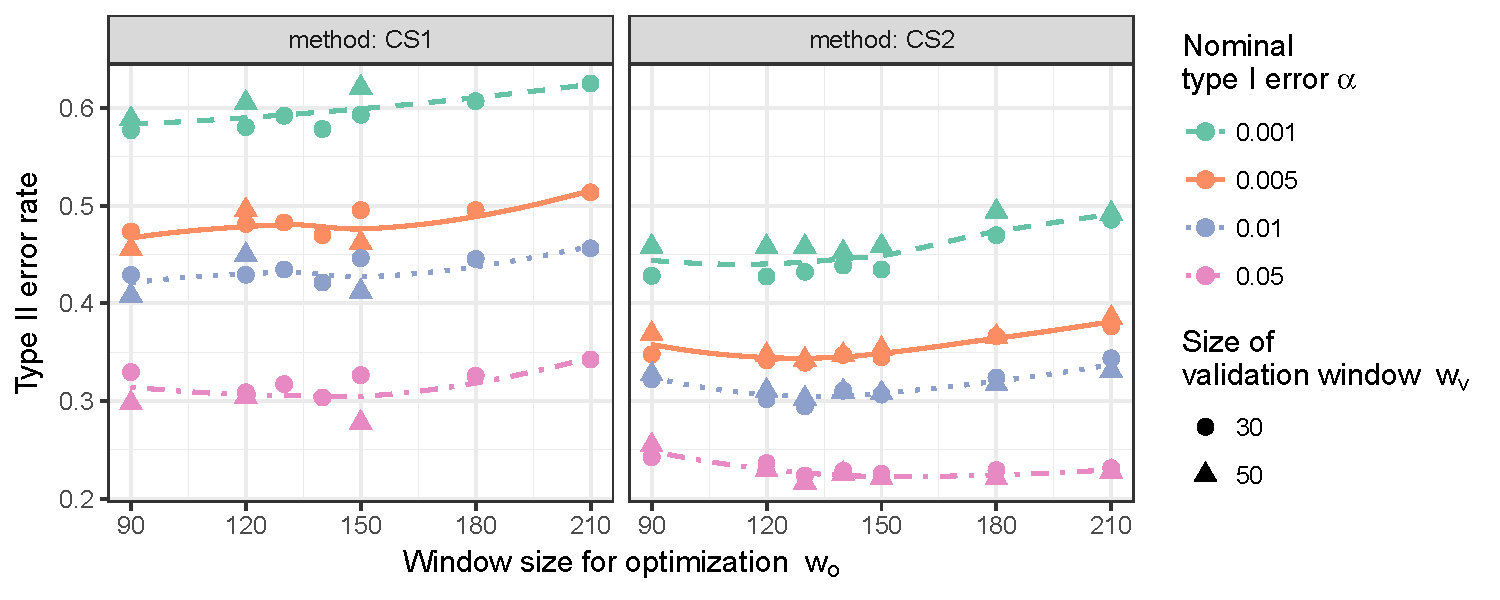
\includegraphics[width=0.9\textwidth]{figures/type2-1} 

}

\caption{Type II error rates observed across a range of window sizes for optimization $w_o$. For a window size of $w_o = 130$ we see a minimum in type II error rate across all type I rates considered. Smaller validation sizes $w_v$ are typically associated with a smaller type II error.}\label{fig:type2}
\end{figure}

\end{appendix}
\end{comment}
\newpage
\bibliographystyle{agsm}
\bibliography{bibliography}

\end{document}
